\documentclass[a4paper,10pt]{article}

\usepackage{fullpage}
\usepackage{graphicx}
\usepackage{amsmath}
\usepackage{amssymb}

% Title Page
\title{Baby Brain Toolkit}
\author{Fbrain ERC project: Computational Anatomy of Fetal Brain}


\begin{document}
\maketitle
\tableofcontents
%\begin{abstract}
%\end{abstract}

\section{Introduction}

BTK stands for Baby Brain Toolkit. This toolkit is developed in the context of
the Fbrain ERC project: ``Computational Anatomy of Fetal
Brain''\footnote{http://lsiit-miv.u-strasbg.fr/miv/index.php?contenu=erc}. 
Studies about brain maturation aim at providing a better understanding of brain
development and links between brain changes and cognitive development. Such
studies are of great interest for diagnosis help and clinical course of
development and treatment of illnesses. Several teams have begun to make 3D maps
of developing brain structures from children to young adults. However, working
out the development of fetal and neonatal brain remains an open issue. This
project aims at jumping over several theoretical and practical barriers and at
going beyond the formal description of the brain maturation thanks to the
development of a realistic numerical model of brain aging.

\subsection{Copyright}
This software is governed by the CeCILL-B license under French law and
abiding by the rules of distribution of free software.  You can  use, 
modify and/ or redistribute the software under the terms of the CeCILL-B
license as circulated by CEA, CNRS and INRIA at the following URL
"http://www.cecill.info". 

As a counterpart to the access to the source code and rights to copy,
modify and redistribute granted by the license, users are provided only
with a limited warranty  and the software's author,  the holder of the
economic rights,  and the successive licensors  have only  limited
liability. 

In this respect, the user's attention is drawn to the risks associated
with loading,  using,  modifying and/or developing or reproducing the
software by the user in light of its specific status of free software,
that may mean  that it is complicated to manipulate,  and  that  also
therefore means  that it is reserved for developers  and  experienced
professionals having in-depth computer knowledge. Users are therefore
encouraged to load and test the software's suitability as regards their
requirements in conditions enabling the security of their systems and/or 
data to be ensured and,  more generally, to use and operate it in the 
same conditions as regards security. 

\subsection{Installation}

\subsubsection{Dependencies}

Baby Brain Toolkit (BTK) depends on:
\begin{itemize}
 \item CMake (www.cmake.org), Tclap (tclap.sourceforge.net), OpenMP (openmp.org), VTK (www.vtk.org), ANN (www.cs.umd.edu/\string~mount/ANN). These libraries can be installed for debian-based distribution using the following command line: \texttt{apt-get install cmake cmake-curses-gui libtclap-dev libgomp1 libvtk5-dev libann-dev}
 \item Insight Toolkit (ITK) version 3.20 (it can be download at www.itk.org). Extract this file (the directory InsightToolkit-3.20 is created). Make another directory where all the build files will be placed, e.g. InsightToolkit-3.20-build:
\begin{verbatim}
mkdir InsightToolkit-3.20-build
cd InsightToolkit-3.20-build
cmake ../InsightToolkit-3.20/
\end{verbatim}
This will bring up the CMake configuration screen. Press \texttt{[c]} for configure and then use \texttt{[t]} to toggle the advanced mode. Make the following changes:
\begin{verbatim}
BUILD_TYPE = Release
ITK_USE_OPTIMIZED_REGISTRATION = ON
ITK_USE_REVIEW = ON
\end{verbatim}
Then press \texttt{[c]} to configure and \texttt{[g]} to generate the make file. Finally, type \texttt{make} at the prompt to obtain the final build of ITK.

\end{itemize}

\subsubsection{Download and compile the BTK sources}
\begin{itemize}
 \item Install Git: this library can be installed for debian-based distribution using the following command line : \texttt{apt-get install git-core}
 \item Get the BTK sources: \texttt{git clone https://github.com/rousseau/fbrain.git }
 \item Then:
\begin{verbatim}
mkdir fbrain-build
cd fbrain-build
cmake ../fbrain
make
\end{verbatim}
\end{itemize}

Most of the programs of the BTK suite use the OpenMP library for multi-threading
purpose. The number of cores used can be tuned using the following command line
(in this example, 4 cores will be used): \texttt{export OMP\_NUM\_THREADS=4}
\section{The BTK pipeline}
BTK allows to implement a pipeline for the processing of fetal images,
i.e. the reconstruction of anatomical and diffusion data, and the final
tractography, all expressed in the same local coordinate system. This
processing can be summarized in the following steps: 1) image conversion, 2) anatomical image reconstruction, 3)
recontruction of the diffusion sequence, 4) registration of diffusion to anatomical data and 5)
tractography.

\subsection{Image conversion}
BTK supports and has been tested by using images in Nifti format
(http://nifti.nimh.nih.gov/nifti-1). However, images are frequently available in
DICOM format and an image conversion is required. This can be performed by using
dcm2nii (http://www.cabiatl.com/mricro/mricron/dcm2nii.html), Slicer or other softwares.

Let say that you have 3 (possibly orthogonal) anatomical images:
\begin{verbatim}
ana01.nii.gz 
ana02.nii.gz 
ana03.nii.gz 
\end{verbatim}

and one set of DWI images: 
\begin{verbatim}
dwi.nii.gz
dwi.bvec 
dwi.bval 
\end{verbatim}

Please check that images are not flipped.\\

\underline{NOTE}: The set of three files .nii.gz, .bvec, and .bval used to
describe a DW sequences are represented in BTK just by the basename (``dwi'' in
the previous example), and the sequences must be provided in this way to the
different applications. This allows to have shorter command lines and a the use
of consistent filenames.

\subsection{Anatomical image reconstruction}
Anatomical image reconstruction can be performed by using \textbf{btkImageReconstruction} (Section
\ref{subsec:ana_rec})\footnote{Best results are obtained by using a mask for each anatomical image. Such image masks can be easily created using ITKSnap for instance.}, followed by a re-orientation procedure using \textbf{btkSetStandardCoorSystem} and \textbf{btkReorientImageToStandard} (Section \ref{sec:utilities})\footnote{Note that the landmarks file is obtained using external software (Slicer). Please see Section \ref{sec:utilities} for details about this step.}:

\begin{verbatim}
 
btkImageReconstruction -i ana01.nii.gz -i ana02.nii.gz -i ana03.nii.gz 
                       -m ana01_mask.nii.gz -m ana02_mask.nii.gz -m ana03_mask.nii.gz
                       -o ana3D.nii.gz --mask

btkSetStandardCoorSystem -i ana3D.nii.gz -o ana3D_standard.nii.gz -d 3
btkReorientImageToStandard -i ana3D_standard.nii.gz -o ana3D_oriented.nii.gz -l landmarks.fcsv

\end{verbatim}



\subsection{Reconstruction of the diffusion sequence}
To reconstruct diffusion data, you want to follow the steps described in
Section \ref{subsec:diff_rec}. The use of two applications is required here:
\textbf{btkGroupwiseS2SDistortionCorrection} and
\textbf{btkRBFInterpolationS2S}.

\subsection{Registration of diffusion to anatomical data}
This can be performed by using \textbf{btkRegisterDiffusionToAnatomicalData}
(Section \ref{subsec:ana_rec})

\subsection{Tractography}
If you have followed the previous steps correctly, at this point you should
have the reconstructed anatomical and diffusion data spatially aligned, and
ready to perform the tractography. To do this, BTK provides
\textbf{btkTractography} (Section \ref{sec:utilities})

\section{Applications}

\subsection{Denoising}

\begin{description}
 \item[btkNLMDenoising] This program applies a non-local mean filter to a 3D image for denoising purpose. Usage: \texttt{-i input\_image\_filename -o output\_image\_filename}. The best results are usually obtained by using a mask (or a padding value).
\end{description}

\begin{description}
 \item[btkNLMDenoising4DImage] This program applies a non-local mean filter to each 3D image of a 4D image, for denoising purpose. Usage: \texttt{-i input\_image\_filename -o output\_image\_filename}. The best results are usually obtained by using a mask (or a padding value).
\end{description}


\subsection{Anatomical reconstruction}
\label{subsec:ana_rec}
\begin{description}
 \item[btkImageReconstruction] This program allows to obtain a
high-resolution image from a set of low-resolution images, typically
axial, coronal, and sagital acquisitions~\cite{Rousseau2006}. \\\\
Minimal usage: \texttt{btkImageReconstruction -i image1 $\cdots$ -i imageN -o
output --box}. 

Recommended usage: \texttt{btkImageReconstruction -i image1 $\cdots$ -i imageN
-m mask1 $\cdots$ -m maskN -o output --mask}. The use of a mask provide
better results since it allows an accuratelly estimation of the initial
transform, and constrains the registration to the region of interest.

The full list of optional parameters of the method can be obtained by
\texttt{btkImageReconstruction --help}

\end{description}

\subsection{Reconstruction of DW sequences}
\label{subsec:diff_rec}
The reconstruction of diffusion-weighted (DW) sequences aims at
obtaining a sequence corrected for fetal moving and eddy-current distortions.
This can be performed in BTK by using the two following applications. 
\begin{description}
\item[btkGroupwiseS2SDistortionCorrection] It performs a groupwise
slice-by-slice registration of the image components of the sequence.

Minimal usage: \texttt{btkGroupwiseS2SDistortionCorrection -i input.nii
-g gradients\_in.bvec -o output.nii -c gradients\_out.bvec -t
pathToTransforms}.

\begin{itemize}
 \item[-i] input sequence
 \item[-g] gradient table for the input sequence
 \item[-o] output sequence 
 \item[-c] gradient table for the output sequence
 \item[-t] folder to save the transformation files
\end{itemize}

The slice-by-slice transform for a given DW image is saved as a set of $N$
transforms in ITK format, with $N$ the number of slices in the image.

NOTE: For slice registration, 20\% of the samples are used for computing the
image metric. As the region of interest of the slice can be small, this number
of samples might be insufficient to compute the metric accurately. However,
this percent of samples has been sufficient for the tested sequences. 

\item[btkRBFInterpolationS2S] It performs an interpolation of scattered data
generated from the application of slice-by-slice transforms. To this end,
radial basis functions are used. By default, the output has isotropic
voxels of size equal to the in-plane resolution of the input.

Minimal usage: \texttt{btkRBFInterpolationS2S -i input.nii -g gradients.bvec
-m mask.nii -o output.nii -t pathToTransforms}.

\begin{itemize}
 \item[-i] input sequence
 \item[-g] gradient table for the input sequence
 \item[-m] mask for the B0 image
 \item[-o] output sequence 
 \item[-t] folder with the transformations generated by
\texttt{btkGroupwiseS2SDistortionCorrection}
\end{itemize}

\end{description}


\subsection{Tractography}
\label{subsec:tracto}
    \subsubsection*{Standard usage}
        Suppose you want to perform a tractography on a diffusion weighted MRI dataset. You should have a dwi image, the corresponding gradient vectors' coordinates, a mask of the brain white matter and a label image of the seeds. Assume this data is stored in files named repsectively for instance \texttt{data.nii.gz}, \texttt{data.bvec}, \texttt{mask.nii.gz} and \texttt{seeds.nii.gz}. The tractography is accomplished by the command below.
            \begin{quote}
                \texttt{btkTractography -d data.nii.gz -g data.bvec -m mask.nii.gz -l seeds.nii.gz}
            \end{quote}
        When the program terminates its task, the probability connection map and the fibers estimation are saved in files respectively named \texttt{map.nii.gz} and \texttt{fibers.vtk}. The connection map is a volume image of probability intensities (\texttt{i.e.} intensities between 0 and 1) with the same origin, orientation and spacing as the diffusion weighted image. The fibers are polygonal data of VTK library in world coordinates. The standard pipeline of the program is shown in Fig.~\ref{btkTractography-fig:standard-pipeline}.
            \begin{figure}
                \centering
                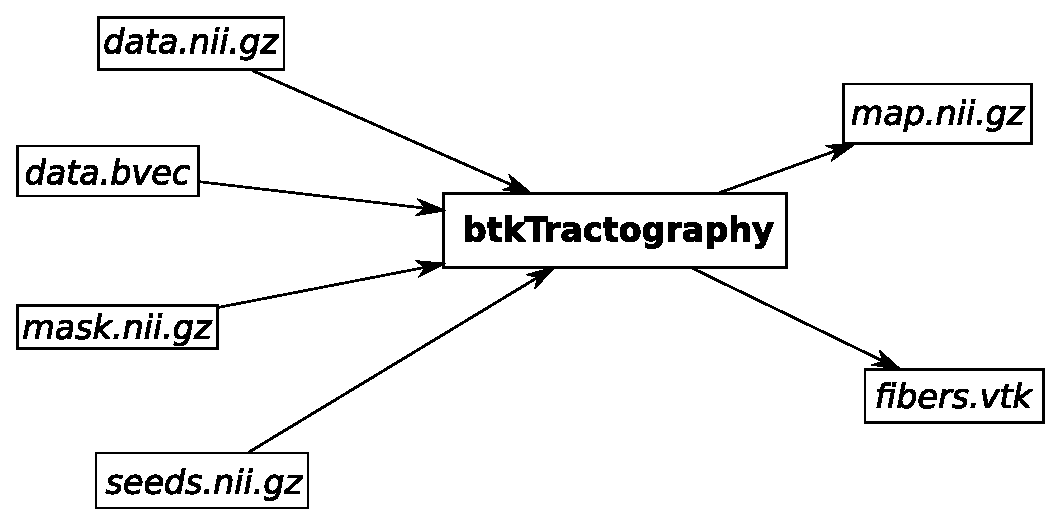
\includegraphics[width=0.6\textwidth]{btkTractographyPipeline}
                \caption{Standard pipeline of the btkTractography program.}
                \label{btkTractography-fig:standard-pipeline}
            \end{figure}

    \subsubsection*{Advanced usage}
        In addition to standard arguments of \texttt{btkTractography} program, there are some other parameters that let you to alter algorithm's behaviour. These options can be classified into three groups : model's options, constraints on trajectory and filter's options. The first group options allow you to tweak the model (for more details about it, please refer to~\cite{descoteaux_regularized_2007}). The second group options let you to control the particle's trajectory. These options provide prior informations to the algorithm. The last group options are dedicated to the particle filter control.

        Since the default parameters values may work in the most of cases, they are optional. A list is of optional features is avaible by using the command
            \begin{quote}
                \texttt{btkTractography -\hspace{0.1mm}-help}
            \end{quote}
        and program's arguments are much more described below.


    \subsubsection*{Model's order}
        The model's order (i.e. the spherical harmonics' order) can be specified by the option
            \begin{quote}
                \texttt{-\hspace{0.1mm}-model\_order <order>} \enspace ,
            \end{quote}
        for \texttt{order}$\;\in\{2,4,6,8\}$. The default value is 4. For more details, please refer to~\cite{descoteaux_regularized_2007}.

    \subsubsection*{Model's regularization}
        A Laplace-Beltrami regularization coefficient is used to assume a better estimation of the model. This coefficient can by manually modified by the option
            \begin{quote}
                \texttt{-\hspace{0.1mm}-model\_regularization <coefficient>} \enspace ,
            \end{quote}
        for \texttt{coefficient}$\;\in\mathbb{R}$. The default value is set as 0.006. For more details, please refer to~\cite{descoteaux_regularized_2007}.

    \subsubsection*{Displacement step size}
        The displacement step size of a moving particle can ben adjusted as you want by using the option
            \begin{quote}
                \texttt{-\hspace{0.1mm}-step\_size <length>} \enspace ,
            \end{quote}
        where \texttt{length}$\;\in\mathbb{R}_+^*$. Note that this option is expressed in~\texttt{mm}. The default value is fixed at 0.5~\texttt{mm}.
        By setting a big step size, the particles will move quickly. So the biger is the step, the faster the algorithm will finish, but as shown by Fig.~\ref{tracto-fig:stepSize}, some informations may be missed and the particle's trajectories may overshoot the ground truth, resulting in a bad estimation.

        \begin{figure}
            \centering
            
\includegraphics[height=0.1\textheight]{stepSize}
            \caption{Effect of the step size option on a particle's trajectory. With a large step size (right), the particle may overshoot the trajectory of the ground truth.}
            \label{tracto-fig:stepSize}
        \end{figure}


    \subsubsection*{Angular threshold}
        An angular threshold prevent a particle to return back. This option has to be expressed in radian and can bet set by
            \begin{quote}
                \texttt{-\hspace{0.1mm}-angular\_threshold <angle>} \enspace ,
            \end{quote}
        where \texttt{angle}$\;\in]0,2\pi[$. The default value is set as a $\tfrac{\pi}{3}$ angle.
        As illustrated in two dimensions in Fig.~\ref{tracto-fig:angleThreshold}, an angle threshold is used to define an allowed area for successive sampled directions. This can be seen as a global curvature parameters on trajectories. A small angle defines trajectories with a small curvature. This is a prior information on ground truth trajectory.

        \begin{figure}
            \centering
            
\includegraphics[height=0.1\textheight]{angleThreshold}
            \caption{An angle threshold allows the algorithm to sample successive direction only in the cone defined by this angle. This illustration show the principle in two dimensions.}
            \label{tracto-fig:angleThreshold}
        \end{figure}


    \subsubsection*{Rigidity}
        The rigidity option controls how much you want the particles to have straight trajectory. You can adjust it by
            \begin{quote}
                \texttt{-\hspace{0.1mm}-curve\_constraint <rigidity>} \enspace ,
            \end{quote}
        where \texttt{rigidity}$\;\in\mathbb{R}_+^*$. The default value is fixed at 30.
        This value correspond to a concentration parameter of a von Mises-Fisher density probability used in the prior density of the system. As Fig.~\ref{tracto-fig:concentration} illustrates locally in two dimensions, a high value leads to a straight trajectory.

        \begin{figure}
            \centering
            
\includegraphics[height=0.1\textheight]{concentration}
            \caption{Local effect of rigidity parameter on a particle's trajectory. This parameter helps to ``attract'' the current displacement vector in the direction of the previous displacement vector of a particle. It correspond to a concentration paramter of a von Mise-Fisher density probability used in the prior density of the system. For instance, a rigidity of 0 leads to an equiprobable distribution, whereas a rigidty tending to infinity leads to a distribution focused on a point.}
            \label{tracto-fig:concentration}
        \end{figure}


    \subsubsection*{Number of particles}
        The number of particles in the system is set by the option
            \begin{quote}
                \texttt{-\hspace{0.1mm}-number\_of\_particles <number>} \enspace ,
            \end{quote}
        where \texttt{number}$\;\in\mathbb{N}^*$. By default, the algorithm will use 1000 particles.
        A poor number of particles leads to a short computation time and a poor estimation. A large number of particles leads to a long computation time and a good estimation. In general, the default number of particles is a good compromise between computation time and estimation.


    \subsubsection*{Resampling threshold}
        This option modify the resampling threshold of the system. When the number of effective particles in the system falls below this resampling threshold, the particles are resampled according a multinomial resampling. It can be adjust by
            \begin{quote}
                \texttt{-\hspace{0.1mm}-resampling\_threshold <percent>} \enspace ,
            \end{quote}
        where \texttt{percent}$\;\in[0,1]$ is the percent of minimal effective particles in the system.
        A low threshold value will result in an inefficient algorithm because the particles with low weight are not are not often eliminated. Conversely, a high threshold value leads to a bad estimation because the search space will not be explored enough.

\section{Utilities}
\label{sec:utilities}

\begin{description}

\item[btkModifyImageUsingLookUpTable] This program modifies one image using a
look up table defined in a ascii file (2 columns, one for the original values,
one for the final values). Usage: \texttt{-i input\_image\_filename -t
input\_table\_filename -o output\_image\_filename}
  

\item[btkNrrdToNifti] This program convert an image from Nrrd file (*.nhdr and *.nrrd) to a Nifti file (*.nii or *.nii.gz). The conversion of a DWI image is possible by using the option \texttt{-d}. Usage: \texttt{-i input.nhdr -o output.nii.gz}. Usage for DWI sequence: \texttt{-i input.nhdr -o output.nii.gz -g gradients.bvec -d}.

\item[btkNiftiToNrrd] This program convert a diffusion sequence in nifti
format\footnote{Currently there is no nifti standard for DWI, so DW images are
saved as a standard nifti sequence and two text files containing the b-values
(.bval) and the gradient directions (.bvec).} (*.nii, *.nii.gz) to the nrrd
format (*.nhdr). 

Usage: \texttt{-i input.nii -b bvalues.bval -g gradients.bvec -o output.nhdr
}

The list of optional parameters can be obtained by \texttt{btkNiftiToNrrd
--help}

\item[btkSetStandardCoorSystem] It transforms an image to a coordinate
system with identity direction and origin at the center of the image
(by default, a linear interpolation is used).

Usage: \texttt{btkSetStandardCoorSystem -i image -o output -d 3}. The argument
$-d$ specifies the image dimension. 

For diffusion sequences, the command line changes to provide the gradient
table, which must be modified accordingly.

Usage: \texttt{btkSetStandardCoorSystem -i image -o output -d 4 -g
gradients.bvec}\\
\texttt{-c outputGradients.bvec}
  
  \item[btkReorientImageToStandard] Sometimes it is useful
to reorient the image to the standard orientation. This is necessary with fetal
images since in general the fetus is in a random orientation with respect to the
scanner. To do this with BTK, before it is necessary to convert the image
to a coordinate system by using \texttt{btkSetStandardCoorSystem}.

Usage: \texttt{btkReorientImageToStandard -i image -o output -l landmarks}.
\texttt{landmarks} is a text file containing points that define the left-right
and the posterior-anterior directions. The points $l$ and $r$ define the left
$\rightarrow$ right direction, and the points $p$ and $a$ define the posterior
$\rightarrow$ anterior direction. Such file can be easily generated by using
Slicer\footnote{http://www.slicer.org} as follows:

\begin{enumerate}
\item Open the high-resolution image by using the \textit{Volume} module.
\item Toogle on the visibility of all slices in the 3D view. This allows to
identify the left and right sides of the brain in the 2D views.
\item Place the landmarks $l$, $r$, $p$, and $a$ in this order by using
\texttt{[p]}.
\item Save the file (*.fcsv) by using the menu File $\rightarrow$ Save.
\end{enumerate}


\begin{figure}[t]
\centering
\begin{tabular}{ccc}
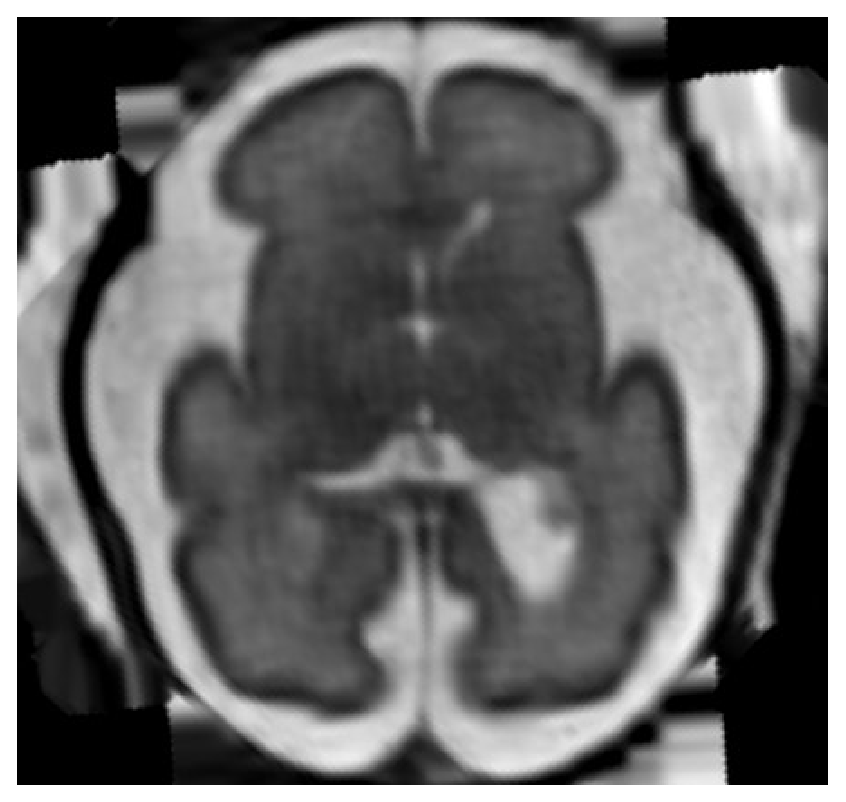
\includegraphics[width=0.3\columnwidth]{hr_axl.eps}&
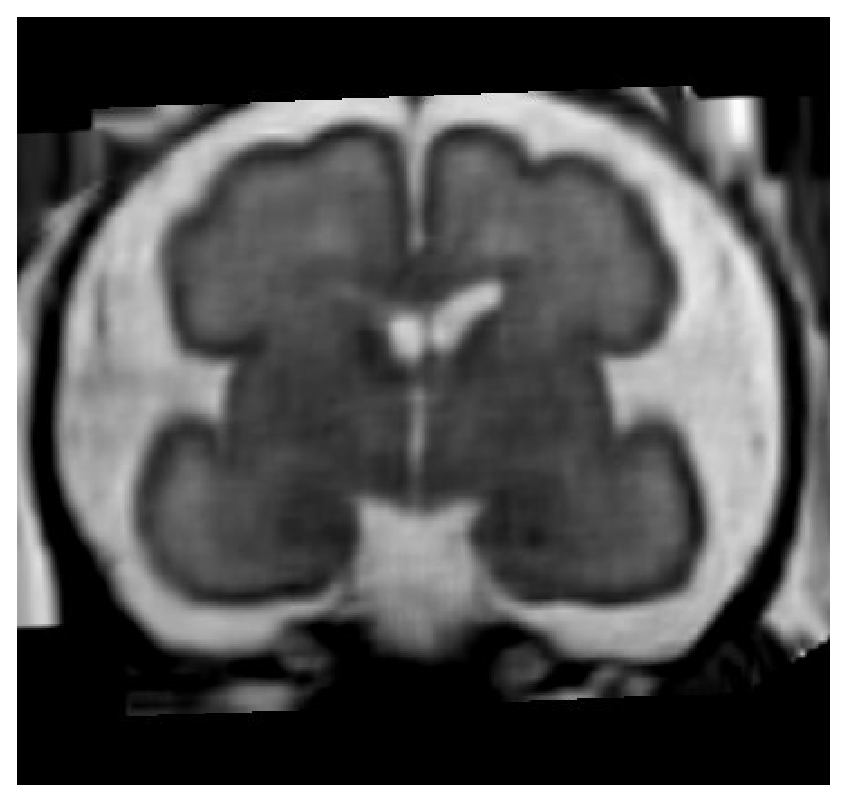
\includegraphics[width=0.3\columnwidth]{hr_cor.eps}&
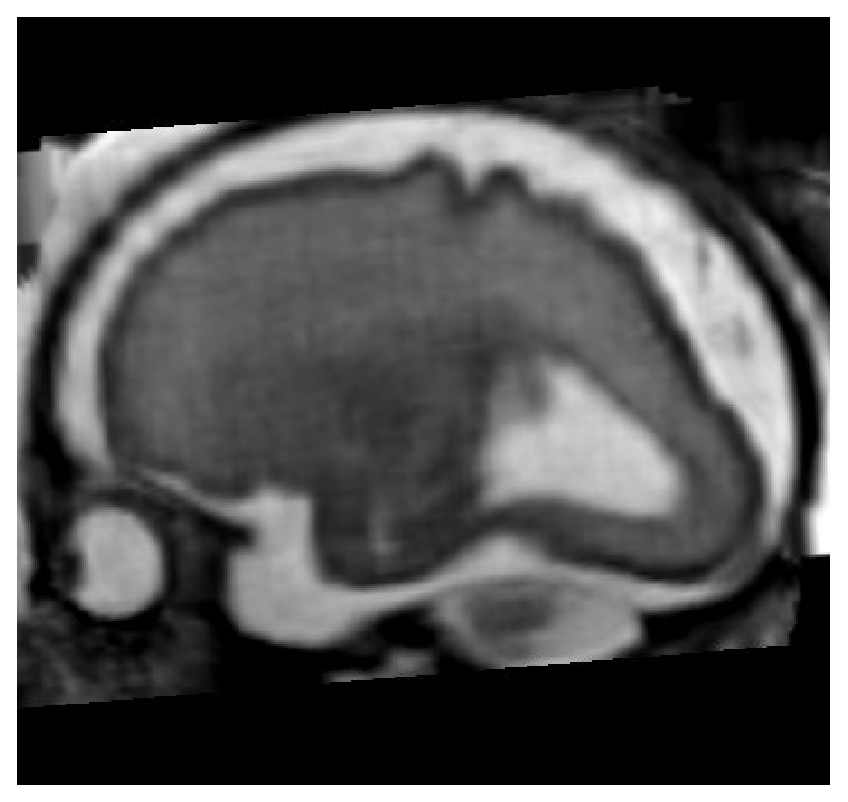
\includegraphics[width=0.3\columnwidth]{hr_sag.eps}\\
{(a)}&{(b)}&{(c)}\\
\end{tabular}
\caption{Example of an anatomical reconstruction of a fetal brain by using
\texttt{btkImageReconstruction}. (a) axial, (b) coronal, and (c) sagital view.}
\label{fig:reconstruction}
\end{figure}

\begin{figure}[t]
\centering
\begin{tabular}{cc}
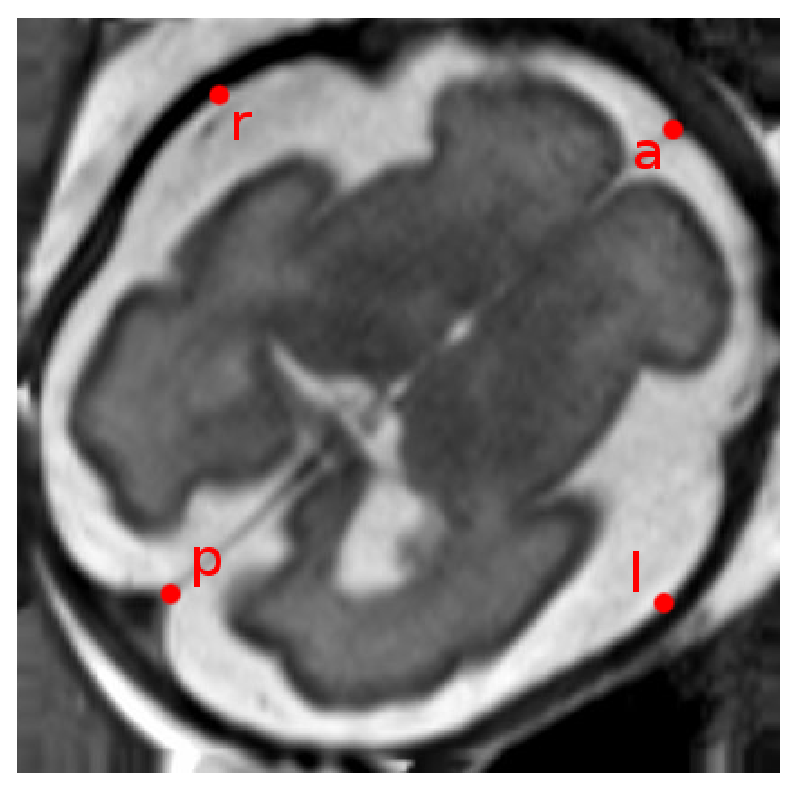
\includegraphics[width=0.35\columnwidth]{lmks_axial.eps}&
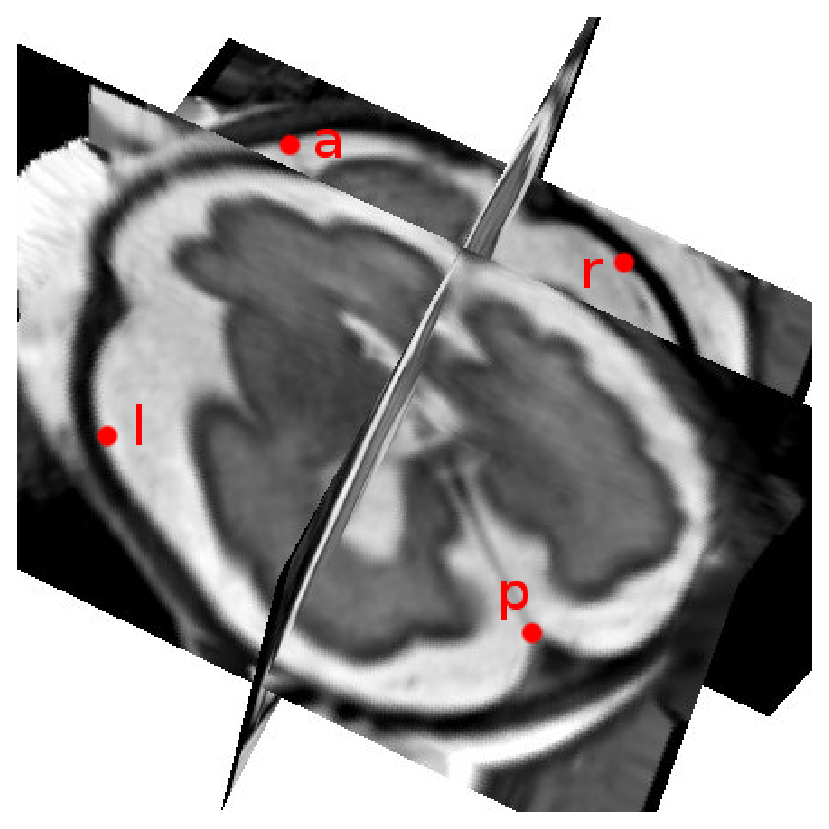
\includegraphics[width=0.35\columnwidth]{lmks_3D.eps}\\
{(a)}&{(b)}\\
\end{tabular}
\caption{Placement of landmarks by using Slicer. (a) axial slice, (b) 3D view.}
\label{fig:landmarks}
\end{figure}

  \item[btkReorientDiffusionSequenceToStandard] Reorients a DW sequence
to the standard orientation. This is necessary with fetal images since the fetus
is in a random orientation with respect to the scanner. This is particularly
important in DWI because colormaps lack of significance, which makes difficult
the identification of specific bundles 

Usage: \texttt{btkReorientDiffusionSequenceToStandard -i image -g
gradients.bvec -l landmarks -o output -c gradients\_corr.bvec}.

\texttt{landmarks} is a landmarks file obtained as explained above.
\texttt{gradients\_corr.bvec} is a text file containing the corrected
gradient table.

\item[btkCropImageUsingMask] This program crops one (3D or 4D) image using a 3D mask. Usage: \texttt{-i input\_image\_filename -m
input\_mask\_filename -o output\_image\_filename -d 3}, where '-d' is the dimension of the input image (by default 3).

\end{description}


\section*{Acknowledgment}
\small{The research leading to these results has received funding from the
European Research Council under the European Community’s Seventh Framework
Programme (FP7/2007-2013 Grant Agreement no. 207667).}

\bibliographystyle{plain}
\bibliography{btk.bib}

\end{document}
